\newpage
\section{Problem}

The goal of this project is to create a user-friendly application that can generate modern 3D cities, and then export them as \textit{.fbx} files.
\textit{User-friendly} means that users should not need any technical expertise or coding experince to fully utilize the application.
\textit{Modern cities} will in this project be defined as cities that resemble
modern industrialized cities such as New York, Paris, San Francisco, and Tokyo.
Figure \ref{fig:ModernCities} showcases two examples of such modern cities.

\begin{figure}[h!]
  \centering

  \begin{subfigure}[b]{0.48\textwidth}
    \frame{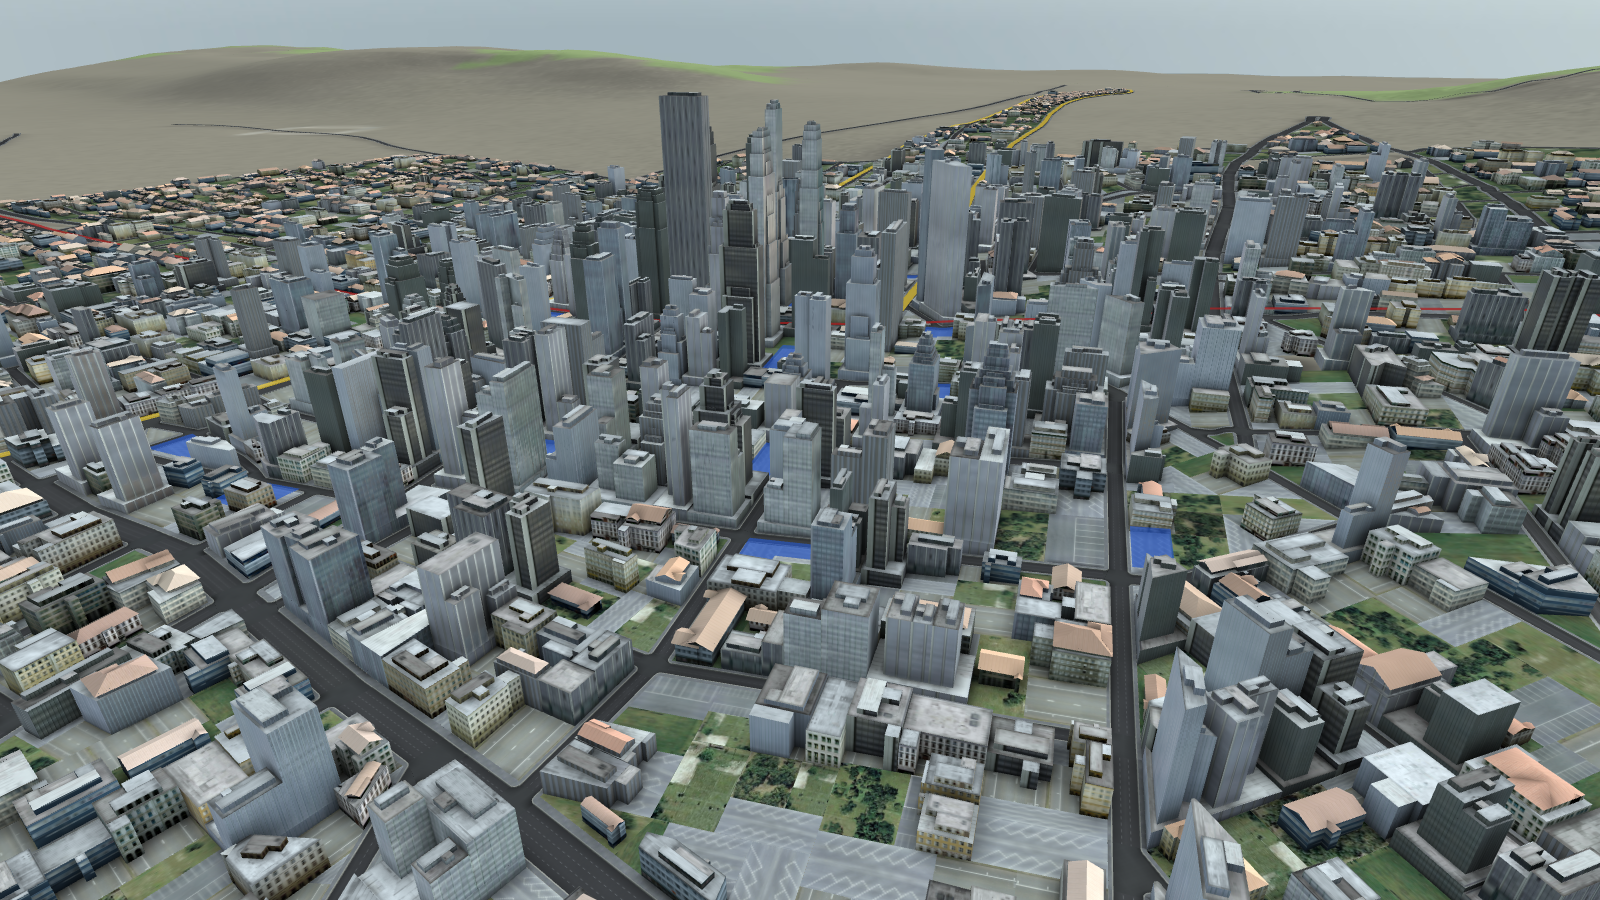
\includegraphics[width=\textwidth]{figure/modern-city.png}}
  \end{subfigure}
  \quad
  \begin{subfigure}[b]{0.48\textwidth}
    \frame{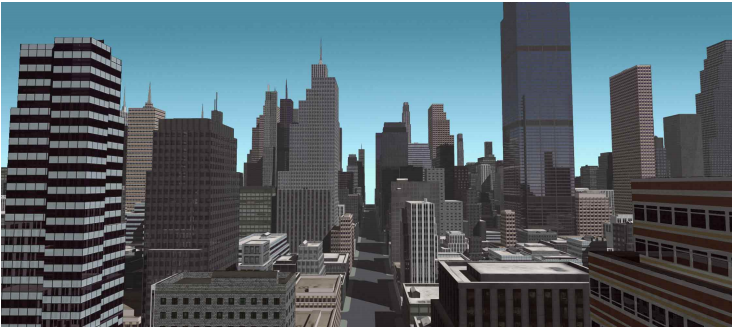
\includegraphics[width=\textwidth]{figure/modern-city2.png}}
  \end{subfigure}

  \caption{Examples of generated modern cities from related works \cite{yoav_and_pascal}\cite{cl3ver}.}
  \label{fig:ModernCities}
\end{figure}

It is worth clarifying that suburban areas and rural areas are also included as
part of such cities.

The scope will be restricted to generating static models that can be exported as \textit{.fbx} files.
Therefore, dynamic content such as simulation of road traffic, day-night cycle,
and pedestrians are all considered out of scope for this project.
The interior of buildings are also considered out of scope.

The primary focus will be put on the generation of roads and buildings as these
are considered the core features of a city.
The terrain's purpose should be to help create natural
settings for these cities to adjust to, and the terrain itself does not need
to have realistic level of detail. Furthermore, the details of roads and
buildings, such as textures and small meshes, are not intended to be made from
scratch. Utilization of free resources online is encouraged to keep the workload
focused on algorithmic problems rather than on 3D modeling.

The user will interact with the application's Graphical User Interface (GUI) in the following way.
\begin{enumerate}
  \item The user specifies the size of the world in terms of a 2D plane.
  \item The user specifies any optional parameters that affect the terrain
    such as sea level.
  \item The user clicks on a button that says ``Generate Terrain'' as many times
    as they like, until they are satisfied with the generated terrain.
  \item The user then selects which region of the generated terrain they want to use in the final model.
  \item The user places population markers on the terrain and specifies how much
    population each marker represents. The user can also specify any optional
    parameters for each marker such as road type.
  \item The user clicks on a button that says ``Generate Roads'' as many times
    as they like, until they are satisfied with the generated road network.
  \item The user clicks on a button that says ``Generate Buildings'' as many times
    as they like, until they are satisfied with the generated buildings.
  \item Finally, when the user is satisfied with the result they can click on a
    button that says ``Export to FBX'' and the the program will save the full
    model as a \textit{.fbx} on the local filesystem.
\end{enumerate}

As a stretch goal, the user should after step 7 be able to select districts of a
city and regenerate those individually. With such a feature in place, the user
would be able to finely adjust the generation to their preference, without the addition of
more mandatory steps.

The problem addressed in this project can be divided into 3 major subproblems:
terrain generation, road generation, and building generation.
Each of the following subsections will go into more detail about these subproblems.

\subsection{Terrain Generation}

e.g. steep hills, rivers, and ocean.
To start with, the algorithm has to create terrain, roads, cells and entities. 

The user will provide a value for the sea level in the form of a number, and we will color the terrain based on the height levels e.g. grasslands near sea level, rocky mountain textures for the taller regions, and snow for top peaks of some of the taller mountains.

\subsection{Road Generation}
\subsection{Building Generation}
